% !TEX encoding = UTF-8 Unicode
%!TEX root = thesis.tex
% !TEX spellcheck = en-US
%%=========================================
\section{Experiment 2}
In this experiment, the aim is to find a good value for parameters related to structural mutation:

\begin{itemize}  
\item Add node probability
\item Remove simple node probability
\item Add link probability
\item Remove link probability
\end{itemize}

\subsection{Configuration}

\begin{center}
\begin{longtable}{p{5cm} p{8.5cm}}
\caption[Experiment configuration]{Experiment configuration} \label{tab:exp1_configuration} \\

\hline \multicolumn{1}{l}{\textbf{Parameter}} & \multicolumn{1}{l}{\textbf{Value}} \\ \hline 
\endfirsthead

\multicolumn{2}{c}%
{{\bfseries \tablename\ \thetable{} -- continued from previous page}} \\
\hline \multicolumn{1}{l}{\textbf{Parameter}} & \multicolumn{1}{l}{\textbf{Value}} \\ \hline 
\endhead

\hline \multicolumn{2}{r}{{Continued on next page}} \\ \hline
\endfoot

\hline \hline
\endlastfoot

Number of generations & 50 \\
\midrule
Fitness function & Local similarity, as described in experiment 1 \\
\midrule
Target sound & Drum loop \\
\midrule
Input sound & White noise \\
\midrule
Effect & Distortion and resonant low-pass filter \\
\midrule
Audio features & mfcc\_0, mfcc\_0\_\_derivative, mfcc\_1 \\
\midrule
Number of runs & 400 per configuration \\
\end{longtable}
\end{center}

\subsection{Results and evaluation}
Figure \ref{fig:exp2_add_link_probability} shows that 0.03 is probably the best value while 0.3 is significantly worse. This might mean that the problem at hand is best solved with few or no hidden nodes. An alternative interpretation is that hidden nodes are useful, but that they slow down the search for the ultimate individual, due to increased complexity.

\begin{figure}[h]
    \centering
    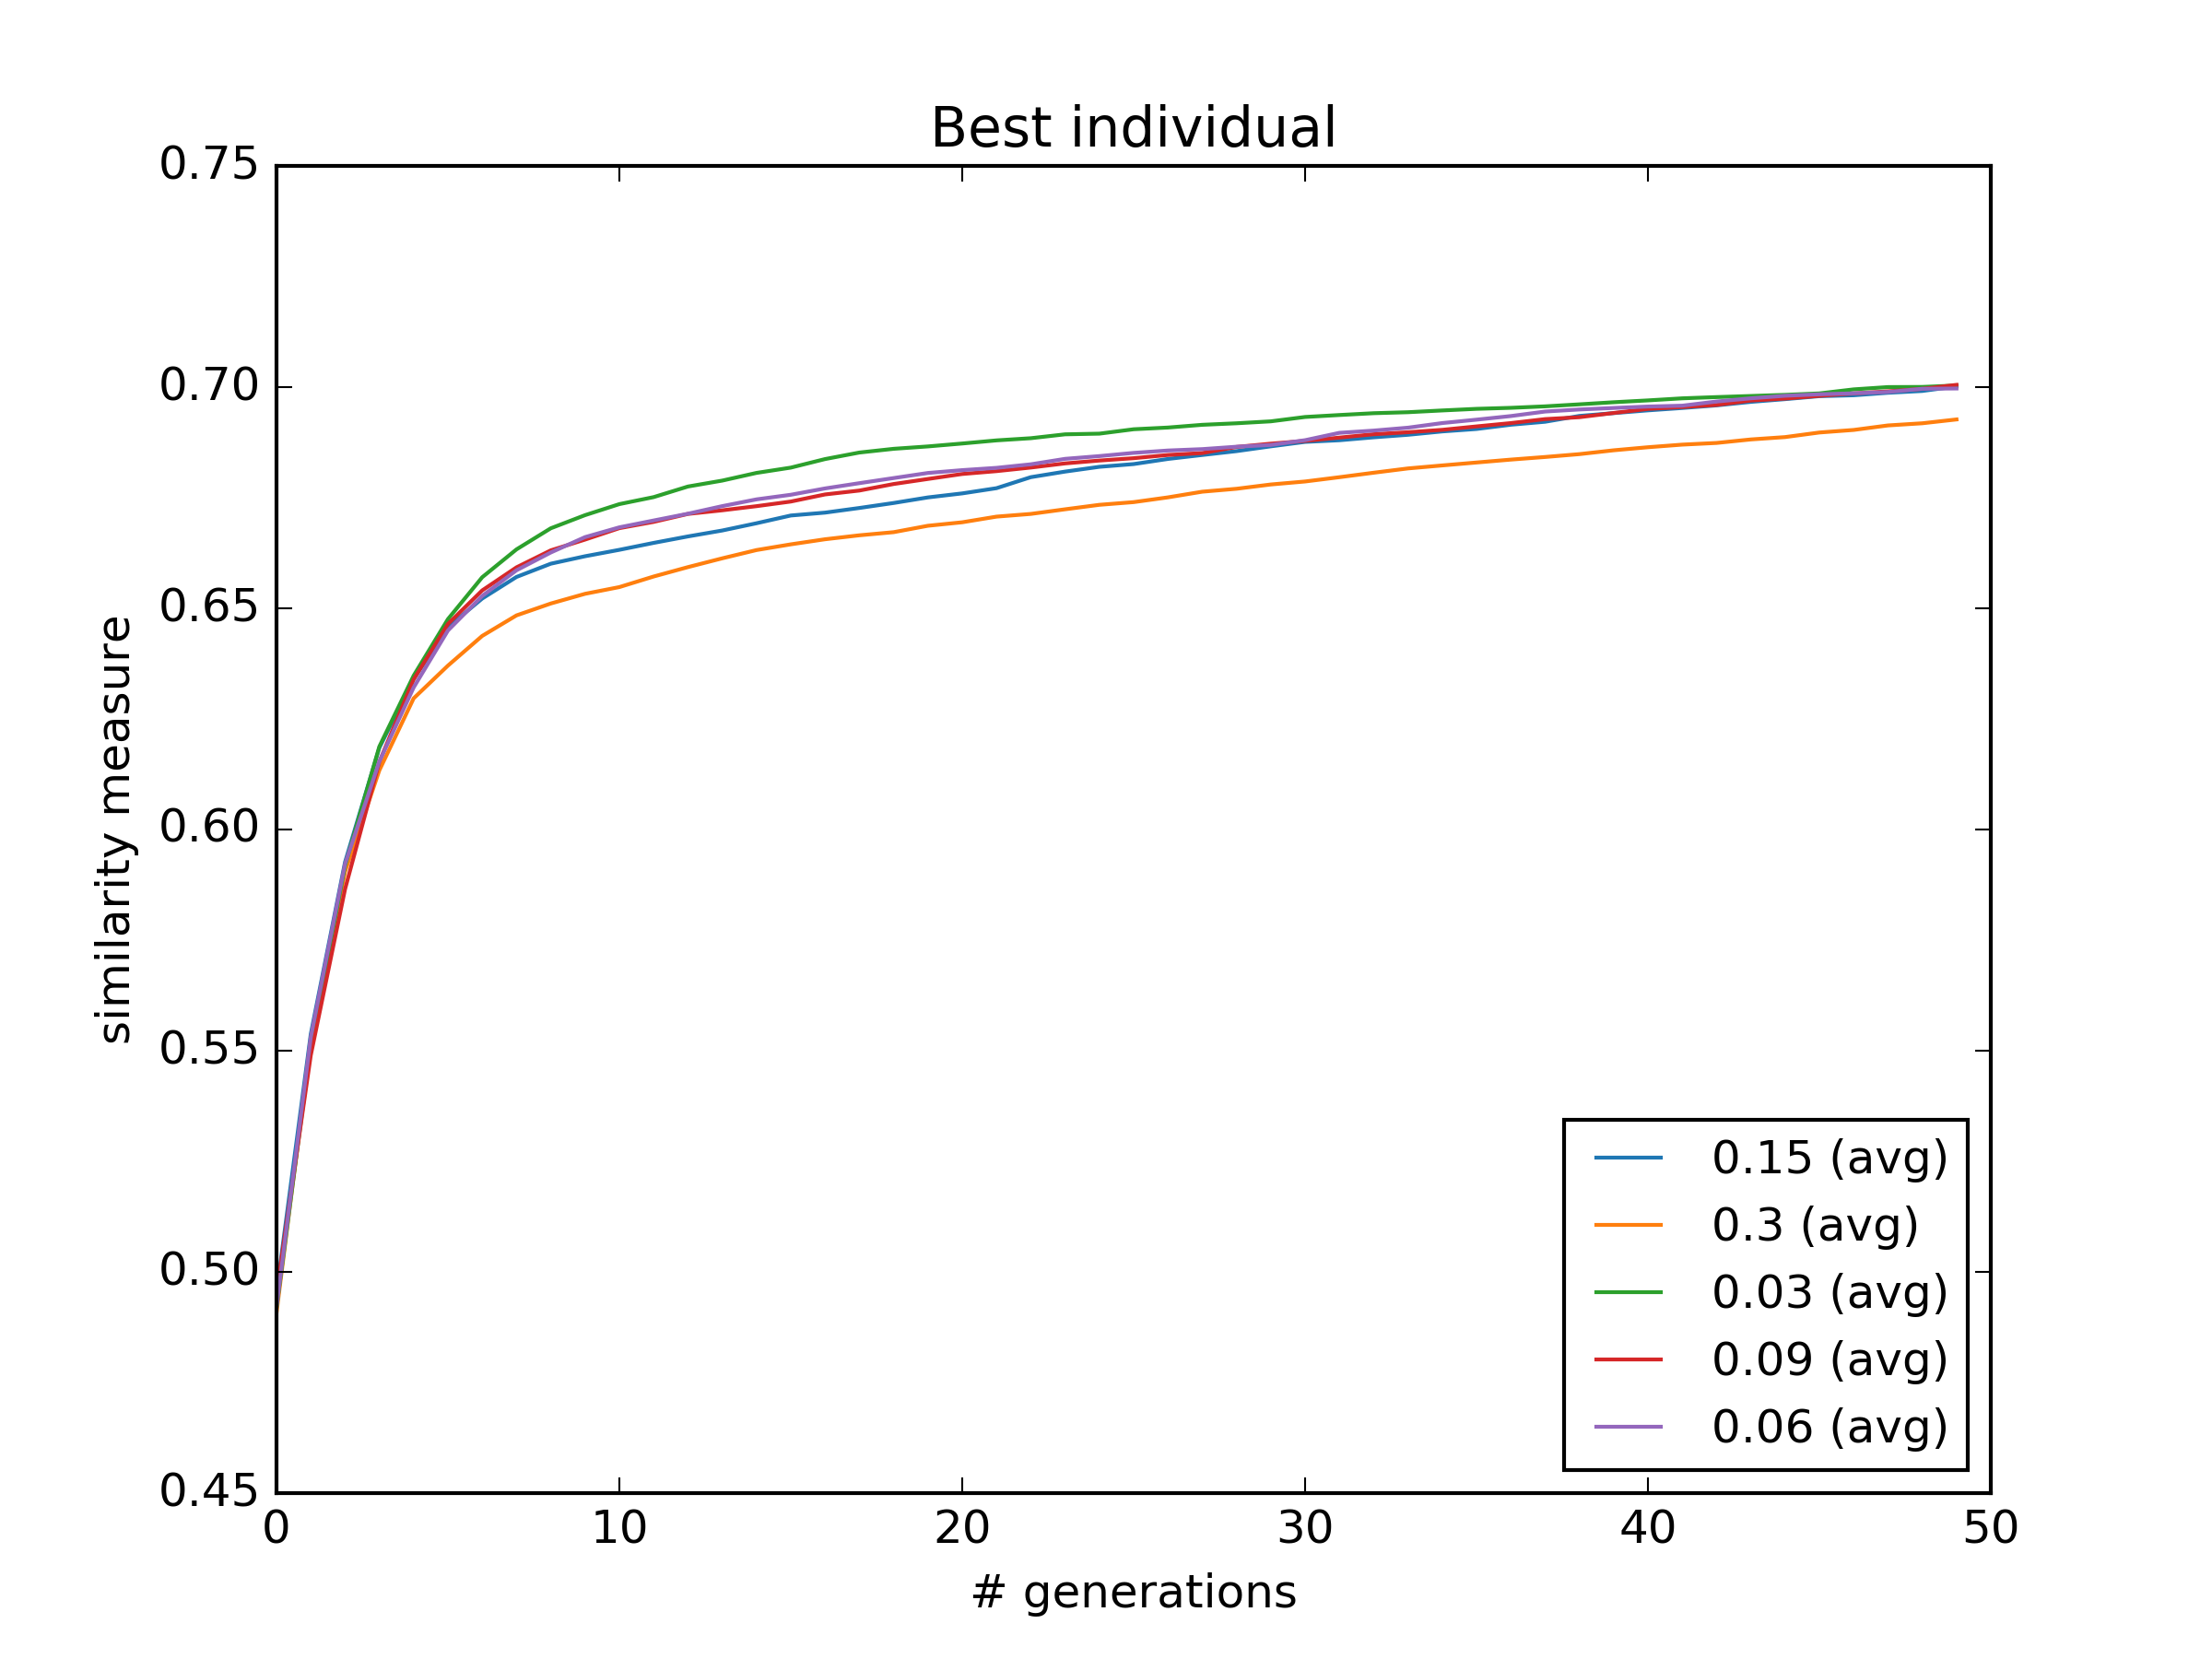
\includegraphics[width=0.99\textwidth]{add_link_probability}
    \caption{Comparison of five different values for the structural mutation parameters}
    \label{fig:exp2_add_link_probability}
\end{figure}

% TODO: Show typical end-result neural networks from all the configurations, to highlight that higher probability builds a larger, more complex network